% !TeX program = lualatex
% !TeX encoding = utf8
% !TeX spellcheck = uk_UA
% !BIB program = bibler

\documentclass[9pt]{beamer}
\usetheme{Electromagnetism}
\usepackage{Electromagnetism}
\usepackage{physics}
\usepackage{tikz}
\usepackage{tikz-3dplot}
\usepackage[outline]{contour} % glow around text
\usepackage{xcolor}
\tikzset{cone/.pic = {
             \draw (-0.5, 0.5) coordinate (-nw) -- ++ (1,-1) coordinate (-se);
             \draw (-0.5,-0.5) coordinate (-sw) -- ++ (1, 1) coordinate (-ne);
             \fill (0,0)  coordinate (-center) circle (0.05);
             \draw (0, 0.5) ellipse (0.5 and 0.05);
             \draw (0,-0.5) ellipse (0.5 and 0.05);
             \coordinate (-top)     at (0, 0.55);
             \coordinate (-north)   at (0, 0.5);
             \coordinate (-south)   at (0,-0.5);
             \coordinate (-bottom)  at (0,-0.55);
            }
            }
\tikzset{middlearrow/.style={
        decoration={markings,
            mark= at position 0.5 with {\arrow{#1}} ,
        },
        postaction={decorate}
    }
}
\newtcolorbox{pict}{
colback=white,
colframe=gray,
boxrule=0.1pt,
left=0pt,
right=0pt,
top=0pt,
bottom=0pt,
sharp corners,
halign=center,
enhanced,drop fuzzy shadow,
hbox,
}

\let\vect\vec
%============================================================================
\title[Лекції електрики та магнетизму]{\huge\bfseries Відносність\\ електричних та магнітних полів. \\ Інваріанти електромагнітного поля}
\subtitle{Лекції з електрики та магнетизму}
\author{Пономаренко С. М.}
%============================================================================
\graphicspath{{pictures/}}

\addtobeamertemplate{frametitle}{}{%
\begin{tikzpicture}[remember picture,overlay]
\node[anchor=north west] at (current page.north west) {\includegraphics[height=1cm]{logo}};
\end{tikzpicture}}


%\titlegraphic{\includegraphics[width=0.25\linewidth]{Einstein}}

\begin{document}
\begin{frame}[plain]
	\tikz [remember picture,overlay]
	\node[anchor=south west, opacity=0.5] at
	(current page.south west)
	%or: (current page.center)
	{\includegraphics[width=0.25\linewidth]{Einstein}};
	\maketitle
\end{frame}


% ============================== Слайд ## ===================================
\begin{frame}{Джерела теорії відносності}{}
	\begin{columns}
		\begin{column}{0.5\linewidth}\small
			Стаття Ейнштейна <<\emph{\color{blue}До електродинаміки рухомих тіл}>> ({\scriptsize \href{https://onlinelibrary.wiley.com/doi/10.1002/andp.19053221004}{Einstein A. Zur Electrodynamik bewegter K{\"o}rper Annalen der Physik, 322, 891-921, 1905.}}) окреслила засади спеціальної теорії відносності, основні постулати якої:

			\bigskip

			\begin{enumerate}\footnotesize
				\item В усіх інерціальних системах відліку фізичні процеси відбуваються однаково.

				      \smallskip

				      \begin{flushleft}\color{red}
					      Закони, що їх описують мають однаковий вигляд  в усіх інерціальних системах відліку.
				      \end{flushleft}

				\item Швидкість світла у вакуумі не залежить від руху джерела або приймача і однакова в усіх напрямах.
			\end{enumerate}

			\begin{center}
				\begin{pict}
					\includegraphics[width=\linewidth]{special_relativity}
				\end{pict}
			\end{center}
		\end{column}
		\begin{column}{0.45\linewidth}
			\begin{center}
				\begin{tikzpicture}[pencildraw/.style={ %
								decorate,
								decoration={random steps,segment length=2pt,amplitude=1pt}
							} %
					]
					\node[align=center,
						preaction={fill=black,opacity=.5,transform canvas={xshift=1mm,yshift=-1mm}},
						pencildraw,draw,fill=white,text width=0.9\linewidth,inner sep=2mm]
					{\includegraphics[width=0.75\linewidth]{zur}};
				\end{tikzpicture}
			\end{center}
			\vspace*{-1em}
			\begin{block}{}\tiny\justifying
				\hspace*{2em}Відомо, що {\color{red}електродинаміка Максвелла --- в сучасному її вигляді --- у застосуванні до рухомих тіл приводить до асиметрії, яка невластива самим явищам}. Пригадаємо, наприклад, електродинамічну взаємодія між магнітом та провідником зі струмом. {\color{red}Спостережуване явище залежить лише від відносного руху провідника і магніту, тоді як, згідно з звичайним уявленням, два випадки, у яких рухається або одне, або інше з цих тіл, повинні бути строго розмежовані}. Справді, {\color{blue}якщо рухається магніт, а провідник знаходиться в спокої, то навколо магніту виникає електричне поле}, що має деяку кількість енергії, яке в тих місцях, де знаходяться частини провідника, породжує струм. {\color{blue}Якщо ж магніт перебуває у спокої, а рухається провідник, навколо магніту немає ніякого електричного поля}; натомість у провіднику виникає електрорушійна сила, якій самій по собі не відповідає жодна енергія, але яка --- при ймовірній тотожності відносного руху в обох випадках, що цікавлять нас --- викликає електричні струми тієї ж величини і того ж напрямку, що і електричне поле в першому випадку.
			\end{block}
		\end{column}
	\end{columns}
\end{frame}
% ===========================================================================






% ============================== Слайд ## ===================================
\begin{frame}{Коваріантність законів фізики}{}
	\begin{block}{}\justifying\small
		Згідно постулату спеціальної теорії відносності, всі інерціальні системи відліку рівноправні, тому закони електродинаміки, як і всі взагалі фізичні явища не змінюються під час переходу від однієї інерційної системи від рахунки $ K $ до будь-якої іншої системи $ K' $, що рухається відносно $ K $ прямолінійно і рівномірно з довільною швидкістю $ \vect{V} $. Однак конкретні фізичні величини змінюються при переході від однієї системи відліку $ K $ до іншої системи $ K' $: результати вимірювання одного й того ж явища у двох різних системах $ K $ та $ K' $, взагалі кажучи, відмінні один від одного.
	\end{block}


	\begin{block}  {}\justifying\small
		Теорія електромагнітних явищ повинна, по-перше, дати відповідь на питання про те, як змінюються значення електромагнітних величин (зокрема, векторів поля $ \Efield $ та $ \Bfield $, густини зарядів і струмів $ \rho $ і $ \vect{j} $ тощо) при зміні системи відліку, і, по-друге, має показати, що із встановленого способу перерахунку фізичних величин з однієї системи відліку до іншої випливає \emph{\color{blue}коваріантність законів електродинаміки}.
	\end{block}

	\begin{alertblock}{}\centering
		Коваріантність законів --- однаковий вигляд у всіх інерціальних системах відліку
	\end{alertblock}

	\begin{alertblock}{}\centering
		Коваріантність законів $ \Rightarrow $ Закони перетворення фізичних величин
	\end{alertblock}
\end{frame}
% ===========================================================================




% ============================== Слайд ## ===================================
\begin{frame}{Перетворення Лоренца}{}

	\begin{columns}
		\begin{column}{0.5\linewidth}
			\begin{block}{}\justifying
				Перетвореннями Лоренца --- це перетворення, яким піддаються координати та час при переході від однієї інерціальної системи відліку до іншої:
				\begin{equation*}\color{red}
					(ct, x, y, z) \rightarrow (ct', x', y', z')
				\end{equation*}
				\begin{tcolorbox}[sharp corners, colframe=blue!50!black, colback=white,  top=0pt]\color{blue}
					\begin{align*}
						c t' & = \frac{c t - \frac{V}{c} x}{\sqrt{1 - \frac{V^2}{c^2}}} = \Gamma \left(ct - \frac{V}{c} x \right), \\
						x'   & = \frac{x - \frac{V}{c} cdt}{\sqrt{1 - \frac{V^2}{c^2}}} = \Gamma (x - V t),                        \\
						y'   & = y, \quad z' = z,
					\end{align*}
				\end{tcolorbox}
				де
				\begin{equation*}\color{red}
					\Gamma = \frac1{\sqrt{1 - \frac{V^2}{c^2}}}.
				\end{equation*}
			\end{block}
		\end{column}
		\begin{column}{0.5\linewidth}
			\begin{pict}
				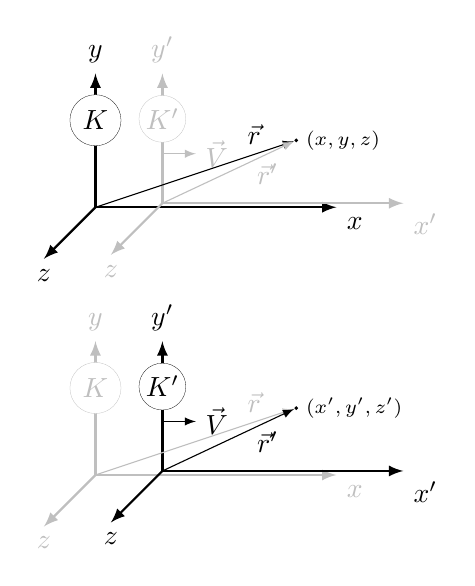
\begin{tikzpicture}[scale=1.7,>=latex]
					\foreach \i in {1,2}{
							\ifnum\i=1
								\edef\cola{gray!50}
								\edef\colb{black}
								\edef\n{0cm}
							\else
								\edef\n{2cm}
								\edef\cola{black}
								\edef\colb{gray!50}
							\fi
							\begin{scope}[yshift=\n]
								\draw[thick,->, \cola] (0,0,0) -- (1.8,0,0) node[anchor=north west]{$x$};
								\draw[thick,->, \cola] (0,0,0) -- node[circle, draw, fill=white, inner sep=2.5pt, pos=0.65, ultra thin] {$ K $} (0,1,0) node[anchor=south]{$y$};
								\draw[thick,->, \cola] (0,0,0) -- (0,0,1) node[anchor=north] {$z$};

								\draw[thick,->, \colb] (0.5,0.03,0) -- +(1.8,0,0) node[anchor=north west]{$x'$};
								\draw[thick,->, \colb] (0.5,0.03,0) -- node[circle, draw, fill=white, inner sep=1pt, pos=0.65, ultra thin] {$ K' $} +(0,0.97,0) node[anchor=south]{$y'$};
								\draw[thick,->, \colb] (0.5,0.03,0) -- +(0,0,1) node[anchor=north] {$z$};

								\draw[->, \colb] (0.5,0.4,0) -- ++(0.25,0,0) node[right] {$ \vect{V} $};

								\node[circle, fill, inner sep=0.5pt] (body) at (1.5,0.5) {};

								\draw[->, thin, \cola] (0,0,0) -- (body) node[above, pos=0.8] {$ \vect{r} $};
								\draw[->, thin, \colb] (0.5,0.03,0) -- (body) node[below, pos=0.8] {$ \vect{r}' $};

								\ifnum\i=1
									\node[right, font=\scriptsize] at (body)
									{$ (x', y', z') $};
								\else
									\node[right, font=\scriptsize] at (body) {$ (x, y, z) $};
								\fi

							\end{scope}
						}
				\end{tikzpicture}
			\end{pict}
		\end{column}
	\end{columns}
\end{frame}
% ===========================================================================




% ============================== Слайд ## ===================================
\begin{frame}{Закон додавання швидкостей}{Перетворення швидкостей}
	\vspace*{-1em}
	\begin{block}{}\small
		Нехай система $ K' $ рухається відносно системи $ K $
		зі швидкістю $ V $ вздовж осі $ x $. Нехай $ v_x = dx/dt $ є компонентою
		швидкості в системі $ K $, a $ v'_x = dx'/dt' $ --- компонента швидкості тієї
		ж частинки у системі $ K' $.
	\end{block}
	\begin{pict}
		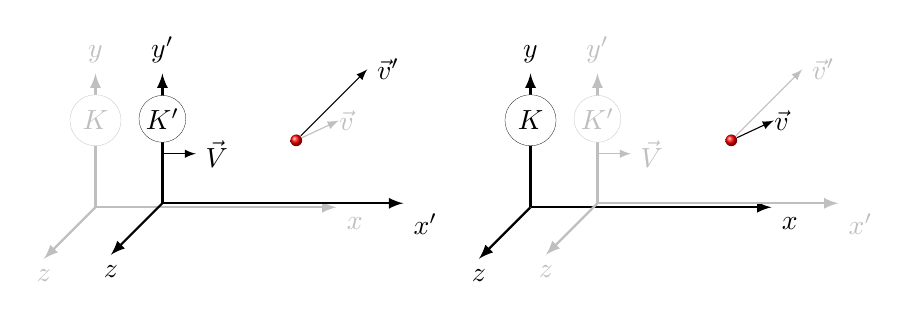
\begin{tikzpicture}[scale=1.7,>=latex]
			\foreach \i in {1,2}{
					\ifnum\i=1
						\edef\cola{gray!50}
						\edef\colb{black}
						\edef\n{0cm}
					\else
						\edef\n{3.25cm}
						\edef\cola{black}
						\edef\colb{gray!50}
					\fi
					\begin{scope}[xshift=\n]
						\draw[thick,->, \cola] (0,0,0) -- (1.8,0,0) node[anchor=north west]{$x$};
						\draw[thick,->, \cola] (0,0,0) -- node[circle, draw, fill=white, inner sep=2.5pt, pos=0.65, ultra thin] {$ K $} (0,1,0) node[anchor=south]{$y$};
						\draw[thick,->, \cola] (0,0,0) -- (0,0,1) node[anchor=north] {$z$};

						\draw[thick,->, \colb] (0.5,0.03,0) -- +(1.8,0,0) node[anchor=north west]{$x'$};
						\draw[thick,->, \colb] (0.5,0.03,0) -- node[circle, draw, fill=white, inner sep=1pt, pos=0.65, ultra thin] {$ K' $} +(0,0.97,0) node[anchor=south]{$y'$};
						\draw[thick,->, \colb] (0.5,0.03,0) -- +(0,0,1) node[anchor=north] {$z$};

						\draw[->, \colb] (0.5,0.4,0) -- ++(0.25,0,0) node[right] {$ \vect{V} $};

						\node[circle, ball color=red, inner sep=1.5pt] (body) at (1.5,0.5) {};
						\draw[->, \colb] (body) -- ++(45:0.75) node[anchor=west,] {$ \vect{v}' $};
						\draw[->, \cola] (body) -- ++(25:0.35) node[anchor=west, inner sep=0pt] {$ \vect{v} $};
					\end{scope}
				}
		\end{tikzpicture}
	\end{pict}
	\begin{equation*}\color{blue}
		v_{x'}  = \frac{v_x - V}{1 - \frac{Vv_x}{c^2}}, \quad
		v_{y'} = \frac{v_y}{\Gamma\left(1 - \frac{Vv_x}{c^2}\right)}, \quad
		v_{z'}  = \frac{v_z}{\Gamma\left(1 - \frac{Vv_x}{c^2}\right)}.
	\end{equation*}

	\begin{block}{}\small\justifying
		Ці формули визначають \emph{\color{blue}перетворення швидкостей}. Вони
		являють собою закон складання швидкостей у теорії
		відносності. У граничному випадку $ c \to \infty $ вони переходять у
		формули класичної механіки $ v_{x'} = v_x - V$,$  v_{y'} = v_y, v_{z'} = v_z $.
	\end{block}
\end{frame}
% ===========================================================================




% ============================== Слайд ## ===================================
\begin{frame}{Просторово-часові поняття}{}

	\begin{block}{}\small\justifying
		\emph{\color{blue}Подія} визначається місцем, де вона відбулась та часом, коли вона відбулась Таким чином, подія, що трапилась з деякою матеріальною частинкою, визначається трьома координатами цієї частинки і моментом часу, коли  відбувається подія.

		\bigskip

		Часто корисно з міркувань наочності користуватись уявним чотиривимірним простором, на осях якого відкладаються три просторові координати і час.

		\bigskip

		В цьому просторі подія зображується точкою $ (ct, x, y, z) $. Ця точка називаються \emph{\color{blue}світовою точкою}.

		\bigskip

		Частинка, що рухається, описує в чотиривимірному просторі траєкторію, яка називається \emph{\color{blue}світовою лінією}.
	\end{block}
	%---------------------------------------------------------
	\vspace{0.5em}
	\begin{minipage}{0.35\linewidth}
		\begin{pict}
			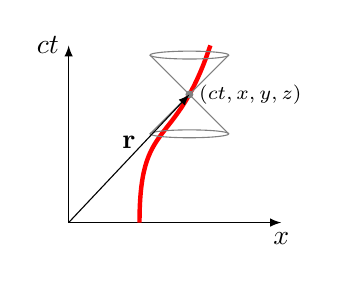
\begin{tikzpicture}[scale=0.45]
				\draw[-latex] (0,0) -- (6,0) node[below] {$x$};
				\draw[-latex] (0,0) -- (0,5) node[left] {$ct$};
				\draw[ultra thick, red] (2,0) ..controls(2,3) and (3,2).. (4,5) coordinate[pos=0.8] (O);
				\node[right, font=\scriptsize] at (O)  {$ (ct, x, y, z) $};;
				\pic[gray] at (O) {cone};
				\draw[-latex] (0,0) -- node[above] {$ \vb{r} $} (O);
			\end{tikzpicture}
		\end{pict}
	\end{minipage}%
	\hfill%---------------------------------------------------------
	\begin{minipage}{0.62\linewidth}\footnotesize
		Сукупність координат події $ (ct, x, y, z) $ можна
		розглядати як компоненти чотиривимірного радіус-вектора
		(або \emph{\color{blue}4-радіус-вектора}).

		\medskip

		\emph{\color{red}Перетворення Лоренца --- це перетворення координат 4-радіус-вектора.}

		\medskip

		Траекторії масивних частинок лежать в середині 4-вимірного \emph{\color{blue}світлового конуса}. Області <<абсолютно майбутнього>> та <<абсолютно минулого>> зображуються тоді двома внутрішніми порожнинами цього конуса. За межами конуса лежать причинно не зв'язані області.
	\end{minipage}
	%---------------------------------------------------------
\end{frame}
% ===========================================================================




% ============================== Слайд ## ===================================
\begin{frame}{Геометрія простору-часу}{}
	\vspace{0em}
	\begin{columns}
		\begin{column}{0.4\linewidth}\centering
			\begin{pict}
				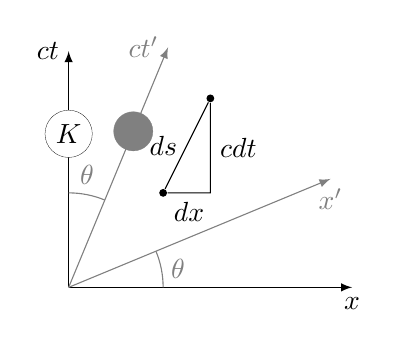
\begin{tikzpicture}[scale=0.6,
					declare function = {alpha=atan{1/2};},]
					\draw[-latex] (0,0) -- (6,0) node[below] {$x$};
					\draw[-latex] (0,0) -- (0,5) node[circle, draw, fill=white, inner sep=2pt, pos=0.65, ultra thin] {$ K $} node[left] {$ct$};

					\draw[-latex, gray] (0,0) -- ++(alpha:6) node[below] {$x'$};
					\draw[-latex, gray] (0,0) -- ++({90-alpha}:5.5) node[circle, draw, fill=white, inner sep=0pt, pos=0.65, ultra thin, gray] {$ K' $} node[left] {$ct'$};
					\draw[gray] (0,2) arc[start angle=90, end angle={90-alpha}, radius=2] node[pos=0.5, above] {$ \theta $};

					\draw[gray] (2,0) arc[start angle=0, end angle=alpha, radius=2] node[pos=0.5, right] {$ \theta $};

					\node[circle, fill, inner sep=1pt] (A) at (2,2) {};
					\node[circle, fill, inner sep=1pt] (B) at (3,4) {};
					\draw (A) -- node[left] {$ ds $} (B) |- node[right, pos=0.25] {$ cdt $} node[below, pos=0.75] {$ dx $} (A);
				\end{tikzpicture}
			\end{pict}
		\end{column}
		\begin{column}{0.6\linewidth}
			<<\emph{\color{blue}Теорема Піфагора}>> в просторі-часі:
			\begin{equation*}%
				\tcbhighmath{
					ds^2 = (cdt)^2 - dx^2 - dy^2 - dz^2
				}
			\end{equation*}

			{\color{blue} $ ds $} називається \emph{\color{blue}інтервалом} між подіями. Інтервал, з формальної математичної точки зору, це відстань між двома точками в просторі-часі.

		\end{column}
	\end{columns}
	\vspace*{0.75em}
	\begin{overprint}
		\onslide<1>
		\begin{center}\color{red}\small
			\begin{align*}
				ds^2 & > 0 \quad \text{--- часоподібний інтервал},       \\
				ds^2 & = 0 \quad \text{--- світлоподібний інтервал},     \\
				ds^2 & < 0 \quad \text{--- просторовоподібний інтервал}.
			\end{align*}
			\begin{enumerate}\scriptsize
				\item \emph{\color{blue}Часоподібний} інтервал між подіями означає, що існує така система відліку, в якій обидві події відбулися в тому самому місці. Що ще важливіше, часовий інтервал між подіями означає, що вони можуть бути причинно пов'язані.
				\item Напрями у просторі-часі, вздовж яких інтервал дорівнює 0, називаються також \emph{\color{blue}ізотропними}. Світло поширюється завжди вздовж ізотропних напрямів.
				\item Події, інтервал між якими \emph{\color{blue}просторовоподібний}, як зазначено вище, не можуть бути причинно пов'язаними, оскільки навіть прямий сигнал, що розповсюджується, мав би для цього рухатися швидше швидкості світла.
			\end{enumerate}
		\end{center}
		\onslide<2>
		Перетворення Лоренца в такій геометрії --- <<\emph{\color{blue}гіперболічний}>> поворот осей координат на кут $ \theta $. Гіперболічний тангенс цього кута є швидкістю $ K' $ системи відліку відносно $ K $:
		\begin{equation*}\color{green!50!black}
			x' = x\ch\theta - ct\sh\theta, \quad ct' = ct\ch\theta - x \sh\theta ,
		\end{equation*}
		де
		\begin{equation*}\color{green!50!black}
			\th\theta = \frac{\sh\theta}{\ch\theta} = \frac{V}{c}, \quad \ch^2 - \sh^2 = 1.
		\end{equation*}

		\vfill

		{\tiny \href{https://uk.wikipedia.org/wiki/\%D0\%9C\%D0\%B0\%D1\%82\%D1\%80\%D0\%B8\%D1\%86\%D1\%8F_\%D0\%BF\%D0\%BE\%D0\%B2\%D0\%BE\%D1\%80\%D0\%BE\%D1\%82\%D1\%83}{перетворення повороту в 3D} }
		\onslide<3>\begin{block}{}
			Як сказав Мінковський: <<Простір сам по собі та час сам по собі поринуть у річку забуття, а залишиться жити лише своєрідний їхній союз>>.
		\end{block}
	\end{overprint}
\end{frame}
% ===========================================================================




% ============================== Слайд ## ===================================
\begin{frame}{4-вектори}{}\small

	%	\vspace*{2.5em}

	\emph{\color{red}4-вектор елементарного зміщення} в просторі-часі
	\begin{equation*}
		{\color{blue} d\vb{s} = (cdt, dx, dy, dz)} = (ds^0, ds^1, ds^2, ds^3)
	\end{equation*}

	\vspace*{-1em}

	\begin{block}{}\scriptsize
		Для зручності запису квадратів 4-векторів вводять два <<сорти>>
		компонент 4-векторів, позначаючи їх верхніми $ A^{\mu} $ та нижніми $ A_{\mu} $ індексами. При цьому
		\begin{equation*}
			A_0 = A^0, \quad A_x = - A^x, \quad A_y = - A^y, A_z = -A^z.
		\end{equation*}
		Величини $ A^{\mu} $ називають контраваріантними, а $ A_{\mu} $ --- \emph{\color{red}коваріантними} компонентами 4-вектора.

		Квадрат 4-вектора елементарного зміщення є інтервалом
		\begin{equation*}
			ds^2 = \sum\limits_{\mu = 0}^3 \sum\limits_{\mu = 0}^3 ds^{\mu} ds_{\mu} = ds^{\mu} ds_{\mu} = (cdt)^2 - dx^2 - dy^2 - dz^2
		\end{equation*}

	\end{block}



	\emph{\color{red}Модуль 4-вектора зміщення}
	\begin{equation*}\color{blue}
		ds = \sqrt{(cdt)^2 - dx^2 - dy^2 - dz^2} = cdt\sqrt{1 - \frac{v^2}{c^2}} = \frac{cdt}{\gamma},\quad \text{де}\quad \gamma = \frac{1}{\sqrt{1 - \frac{v^2}{c^2}}}.
	\end{equation*}

	Вектор \emph{\color{red}4-швидкості}:
	\begin{equation*}\color{blue}
		\vb{u} = c\frac{d\vb{s}}{ds}, \quad u^{ct} = c\frac{cdt}{ds} = c\gamma, u^x = c\frac{dx}{ds} = \gamma v_x, \ldots
	\end{equation*}

	\medskip

	\emph{\color{red}Квадрат 4-швидкості}
	\begin{equation*}\color{blue}
		\vb{u}^2 = u^{\mu}u_{\mu} = \gamma^2 c^2 - \gamma^2 v_x^2 - \gamma^2 v_y^2 - \gamma^2 v_z^2 = \gamma^2(c^2 - v^2) = c^2\gamma^2 \left( 1- \frac{v^2}{c^2} \right) = c^2
	\end{equation*}


\end{frame}
% ===========================================================================




% ============================== Слайд ## ===================================
\begin{frame}{4-вектори}{4-імпульс}
	\emph{\color{red}Вектор 4-імпульсу}:
	\begin{equation*}\color{blue}
		\vb{p} = m\vb{u}
	\end{equation*}

	\emph{\color{red}Компоненти 4-імпульсу}
	\begin{equation*}\color{blue}
		p^0 = mc\gamma = \frac{E}{c}, \quad p^1 = mv_x\gamma, \quad p^2 = mv_y\gamma, \quad p^3 = mv_z\gamma.
	\end{equation*}

	\emph{\color{red}Квадрат 4-імпульсу}
	\begin{equation*}\color{blue}
		\vb{p}^2 = p^{\mu}p_{\mu} = m^2c^2 =  \left( \frac{E}{c} \right)^2 - p^2
	\end{equation*}

	\begin{overprint}
		\onslide<1>
		\begin{block}{Означення 4-вектора}\justifying
			4-вектором називається сукупність чотирьох величин $ (A^0, A^1, A^2, A^3) $, які при перетвореннях чотиривимірної системи координат
			перетворюються як компоненти 4-радіус-вектора:
			\begin{equation*}
				A^{0'} = \Gamma \left( A^{0} - \frac{V}{c} A^{1}\right), \quad A^{1'} = \Gamma \left( A^{1} - \frac{V}{c} A^{0}\right), \quad A^{2'} = A^2, \quad A^{3'} = A^3.
			\end{equation*}
		\end{block}
		\onslide<2>
		\begin{tblr}{
			colspec={cc},
			row{1} = {c},
			row{2-Z} = {mode=dmath},
			hline{1,Z} = {0pt},
					hline{2} = {2pt, blue},
					vline{2} = {2pt, blue},
					hlines
				}
			Для компонент 4-зміщення & Для компонент 4-імпульсу                                                                                \\
			%% --------------------------------------------------------
			cdt' = \frac{cdt - \frac{V}{c}dx}{\sqrt{1 - \frac{V^2}{c^2}}} = \Gamma \left(cdt - \frac{V}{c}dx \right)
			                         &
			\frac{E'}{c} = \frac{\frac{E}{c} - \frac{V}{c}p_x}{\sqrt{1 - \frac{V^2}{c^2}}} = \Gamma \left(\frac{E}{c} - \frac{V}{c}p_x \right) \\
			%% --------------------------------------------------------
			dx' = \frac{dx - \frac{V}{c} cdt}{\sqrt{1 - \frac{V^2}{c^2}}} = \Gamma (dx - V dt)
			                         &
			p_{x'} = \frac{p_x - \frac{V}{c} \frac{E}{c}}{\sqrt{1 - \frac{V^2}{c^2}}} = \Gamma \left(p_x - V \frac{E}{c}\right)                \\
			%% --------------------------------------------------------
			dy' = dy, \quad dz' = dz
			                         &
			p_{y'} = p_y, \quad p_{z'} = p_z                                                                                                   \\
		\end{tblr}
	\end{overprint}



\end{frame}
% ===========================================================================

% ============================== Слайд ## ===================================
\begin{frame}{Перетворення сили}{}
	\begin{alertblock}{}\centering
		Коваріантність законів --- однаковий вигляд у всіх інерціальних системах відліку
	\end{alertblock}

	\begin{center}
		\begin{tblr}{
			colspec={lcc},
			column{2,3}={mode=dmath},
				}
			В системі $ K $
			 & \vect{F} = \frac{d\vect{p}}{dt}
			 & \left(\vect{F}\cdot\frac{\vect{v}}{c}\right) = \frac{d}{dt}\left( \frac{E}{c}\right)
			\\
			В системі $ K' $
			 & \vect{F}' = \frac{d\vect{p'}}{dt'}
			 & \left(\vect{F'}\cdot\frac{\vect{v'}}{c}\right) = \frac{d}{dt}\left( \frac{E'}{c}\right)
		\end{tblr}
	\end{center}

	{\color{blue}
	\begin{align*}
		F_{x'} & = F_x  - \frac{v_y V}{c^2}\Gamma F_{y'} - \frac{v_z V}{c^2}\Gamma F_{z'}, \\
		F_{y'} & = \frac{F_y}{\Gamma\left( 1 - \frac{v_x V}{c^2}\right) },                 \\
		F_{z'} & = \frac{F_z}{\Gamma\left( 1 - \frac{v_x V}{c^2}\right) }
	\end{align*}
	}
\end{frame}
% ===========================================================================





% ============================== Слайд ## ===================================
\begin{frame}{Інваріантність заряду}{}
	\begin{alertblock}{}\centering
		Заряд --- релятивістськи інваріантна величина!
	\end{alertblock}
	\begin{columns}
		\begin{column}{0.5\linewidth}\centering
			Інваріантність заряду
			\begin{equation*}
				\iiint\limits_V \rho\, dxdydz = \iiint\limits_{V'} \rho_0 dx'dy'dz',
			\end{equation*}
			$ \rho_0 $ --- власна густина заряду.

			\medskip

			Лоренцівське скорочення ($ dt = 0 $)
			\begin{align*}
				dx' & = \frac{dx}{\sqrt{1 - \frac{V^2}{c^2}}} = \Gamma dx, \\
				dy' & = dy, \quad  dz' = dz.
			\end{align*}

			\medskip

			Перетворення для густини заряду
			\begin{equation*}\color{blue}
				\rho = \frac{\rho_0}{\sqrt{1 - \frac{V^2}{c^2}}} = \Gamma\rho_0.
			\end{equation*}
		\end{column}
		\begin{column}{0.5\linewidth}\centering
			\begin{pict}
				\begin{tikzpicture}[scale=1.7,>=latex]
					%% ========================================================
					\begin{scope}
						\draw[thick,->, gray!50] (0,0,0) -- (2,0,0) node[anchor=north west]{$x$};
						\draw[thick,->, gray!50] (0,0,0) -- node[circle, draw, fill=white, inner sep=2.5pt, pos=0.65, ultra thin] {$ K $} (0,1,0) node[anchor=south]{$y$};
						\draw[thick,->, gray!50] (0,0,0) -- (0,0,1) node[anchor=north] {$z$};

						\draw[thick,->] (0.5,0.03,0) -- +(2,0,0) node[anchor=north west]{$x'$};
						\draw[thick,->] (0.5,0.03,0) -- node[circle, draw, fill=white, inner sep=1pt, pos=0.65, ultra thin] {$ K' $} +(0,0.97,0) node[anchor=south]{$y'$};
						\draw[thick,->] (0.5,0.03,0) -- +(0,0,1) node[anchor=north] {$z$};

						\draw[->] (0.5,0.4,0) -- ++(0.25,0,0) node[right] {$ \vect{V} $};

						\pgfmathsetseed{3}
						\begin{scope}[shift={(1.5,0.5)}]
							\draw[fill=red!20, ultra thin] plot [smooth cycle, samples=8,domain={1:8}]
							(\x*360/8+5*rnd:0.1cm+0.2cm*rnd);
						\end{scope}
						\node[above=0.4cm, text=gray, font=\scriptsize] at (1.5,0.5) {$ \rho_0 $ --- густина в $ K' $};
					\end{scope}
					%% ========================================================
					\begin{scope}[yshift=-1.8cm]
						\draw[thick,->] (0,0,0) -- (2,0,0) node[anchor=north west]{$x$};
						\draw[thick,->] (0,0,0) -- node[circle, draw, fill=white, inner sep=2.5pt, pos=0.65, ultra thin] {$ K $} (0,1,0) node[anchor=south]{$y$};
						\draw[thick,->] (0,0,0) -- (0,0,1) node[anchor=north] {$z$};

						\draw[thick,->, gray!50] (0.5,0.03,0) -- +(2,0,0) node[anchor=north west]{$x'$};
						\draw[thick,->, gray!50] (0.5,0.03,0) -- node[circle, draw, fill=white, inner sep=1pt, pos=0.65, ultra thin] {$ K' $} +(0,0.97,0) node[anchor=south]{$y'$};
						\draw[thick,->, gray!50] (0.5,0.03,0) -- +(0,0,1) node[anchor=north] {$z$};

						\draw[->, gray!50] (0.5,0.4,0) -- ++(0.25,0,0) node[right] {$ \vect{V} $};

						\pgfmathsetseed{3}
						\begin{scope}[shift={(1.5,0.5)}, xscale=0.5]
							\draw[fill=red!50, ultra thin] plot [smooth cycle, samples=8,domain={1:8}]
							(\x*360/8+5*rnd:0.1cm+0.2cm*rnd);
						\end{scope}
						\node[above=0.4cm, text=gray, font=\scriptsize] at (1.5,0.5) {$ \rho = \frac{\rho_0}{\sqrt{1 - \frac{V^2}{c^2}}} $ --- густина в $ K' $};
					\end{scope}
					%% ========================================================
				\end{tikzpicture}
			\end{pict}
		\end{column}
	\end{columns}

\end{frame}
% ===========================================================================





% ============================== Слайд ## ===================================
\begin{frame}{Перетворення для електричного та магнітного полів}{}
	Нехай в системі $ K $ існує електричне $ \Efield $ та магнітне $ \Bfield $ поля. У системі $ K' $ напруженість $ \Efield' $ та індукція $ \Bfield' $.

	\bigskip

	\begin{overprint}
		\onslide<1>\small
		Скористаємося виразами для сили Лоренца:
		\begin{equation*}
			\vect{F} = q\left( \Efield + \left[ \frac{\vect{v}}{c}\times\Bfield\right] \right) , \quad
			\vect{F}' = q\left( \Efield' + \left[ \frac{\vect{v}'}{c}\times\Bfield'\right] \right)
		\end{equation*}

		Розглянемо $ y $ компоненту
		\begin{equation*}
			F_y = F_{y'}\Gamma\left( 1 - \frac{v_xV}{c^2}\right)
		\end{equation*}
		\begin{equation*}
			E_y + \frac{v_z}{c}B_x - \frac{v_x}{c}B_z = \Gamma\left( 1 - \frac{v_xV}{c^2}\right) \left( E_{y'} + \frac{v_{z'}}{c}B_{x'} - \frac{v_{x'}}{c}B_{z'} \right)
		\end{equation*}
		Виключаючи в цьому рівнянні за допомогою перетворень швидкостей компоненти вектора швидкості, і групуючи доданки біля компонент швидкостей, перепишемо останню рівність у вигляді:
		\begin{equation*}
			\left( E_y  - \Gamma E_{y'} -\Gamma\frac{V}{c}B_{z'}\right) +
			\left( - B_z +\Gamma\frac{V}{c}E_{y'} +\Gamma B_{z'}\right)v_x +
			\left( B_x - B_{x'}\right)v_z = 0.
		\end{equation*}
		Оскільки ця рівність повинна виконуватися за будь-якої швидкості $ \vect{v} $, вирази в круглих дужках повинні дорівнювати нулю. Отже
		\begin{equation*}\color{blue}
			E_y = \Gamma\left( E_{y'} + \frac{V}{c}B_{z'}\right), \quad B_x = B_{x'}, \quad  B_z = \Gamma\left(B_{z'} + \frac{V}{c}E_{y'} \right).
		\end{equation*}
		\onslide<2>
		\vspace*{5em}
		\begin{center}
			Перетворення для електричного та магнітного полів
		\end{center}
		\begin{tcolorbox}[sharp corners, colframe=blue!50!black, colback=white,  top=0pt]
			{ \color{blue}
				\begin{align*}
					E_x = E_{x'},                                         & \quad B_x = B_{x'} \\
					E_y = \Gamma\left( E_{y'} + \frac{V}{c}B_{z'}\right), & \quad
					B_y = \Gamma\left( B_{y'} - \frac{V}{c}E_{z'}\right) ,                     \\
					E_z = \Gamma\left( E_{z'} - \frac{V}{c}B_{y'}\right), & \quad
					B_z = \Gamma\left( B_{z'} + \frac{V}{c}E_{y'}\right)
				\end{align*}
			}
		\end{tcolorbox}

		\vspace*{5em}

		{\tiny \url{https://youtu.be/h7LaQPvzHZo}}
	\end{overprint}
\end{frame}
% ===========================================================================





% ============================== Слайд ## ===================================
\begin{frame}{Інваріанти електромагнітного поля}{}
	\begin{block}{}\justifying\small
		Інваріантами перетворень електромагнітного поля називаються такі величини, складені з векторів поля, які змінюють значення при переході від однієї інерційної системи відліку до іншого.
	\end{block}
	\begin{tcolorbox}[sharp corners, colframe=blue!50!black, colback=white,  top=0pt]
		{\color{blue}
			\begin{align*}
				E^2 - B^2           & = E'^2 - B'^2 = \mathrm{inv},           \\
				\Efield\cdot\Bfield & = \Efield'\cdot\Bfield' = \mathrm{inv}.
			\end{align*}
		}
	\end{tcolorbox}
	\begin{enumerate}\footnotesize
		\item якщо в деякій інерційній системі відліку {\color{red} $ B^2 > E^2 $}  і {\color{blue} $ \Bfield \perp \Efield $}, то можна вибрати таку інерційну систему відліку, де електричне поле відсутнє, а магнітне відмінне від нуля. Якщо $ \Bfield $ не перпендикулярно $ \Efield $, то такої інерційної системи відліку не існує;
		\item  якщо в деякій інерційній системі відліку {\color{red} $ B^2 < E^2 $} і {\color{blue} $ \Bfield \perp \Efield $}, то можна вибрати таку інерційну систему відліку, де магнітне поле відсутнє, а електричне відмінне від нуля. Якщо $ \Bfield $ не перпендикулярно $ \Efield $, то такої інерційної системи відліку не існує;
		\item якщо в будь-якій інерційній системі відліку є тільки електричне поле або тільки магнітне, то при переході до іншої інерційної системи відліку є взагалі кажучи, як електричне, так і магнітне поля, які перпендикулярні один одному {\color{red} $ \Bfield \perp \Efield $};
		\item плоска хвиля, для якої {\color{red} $ E = B $} і {\color{blue} $ \Bfield \perp \Efield $}, у всіх інерційних системах відліку  залишається плоскою хвилею.
	\end{enumerate}{}

	\begin{exampleblock}{}\small
		Якщо в одній системі відліку є лише електричне поле $ \Efield $, чи можна знайти таку систему відліку в якій існує лише магнітне поле $ \Bfield' $?
	\end{exampleblock}
\end{frame}
% ===========================================================================

% ============================== Слайд ## ===================================
\begin{frame}{Електричне поле в рухомій системі відліку}{}
	\begin{exampleblock}{}\centering\small
		Відоме електричне поле $ \vect{E} $ нитки рухомій системі відліку $ K' $. Знайти його величину в нерухомій $ K $ системі відліку.
	\end{exampleblock}
	\vspace*{-1ex}
	\begin{center}
		\begin{pict}
			\begin{tikzpicture}[scale=1.75,>=latex]
				%% ========================================================
				\draw[thick,->, gray!50] (0,0,0) -- (2,0,0) node[anchor=north west]{$x$};
				\draw[thick,->, gray!50] (0,0,0) -- node[circle, draw, fill=white, inner sep=2.5pt, pos=0.65, ultra thin] {$ K $} (0,1,0) node[anchor=south]{$y$};
				\draw[thick,->, gray!50] (0,0,0) -- (0,0,1) node[anchor=north] {$z$};

				\begin{scope}
					\draw[thick,->] (0.5,0.03,0) -- +(2,0,0) node[anchor=north west]{$x'$};
					\draw[thick,->] (0.5,0.03,0) -- node[circle, draw, fill=white, inner sep=1pt, pos=0.65, ultra thin] {$ K' $} +(0,0.97,0) node[anchor=south]{$y'$};
					\draw[thick,->] (0.5,0.03,0) -- +(0,0,1) node[anchor=north] {$z$};

					\draw[->] (0.5,0.4,0) -- ++(0.25,0,0) node[right] {$ \vect{V} $};
					\node [circle, inner sep=0.05cm, ball color=red] (q) at (1.5,0.6,0) {};
					\node[left] at (q) {$ q $};
					\draw[->, red] (q) -- ++(0,0.5) node[above] {$ q\vect{E}' $};

					\begin{scope}% infinite wire
						\def\xstartpos{1}
						\def\ystartpos{0}
						\def\thickness{0.02}
						\def\len{1}
						\draw[fill=red!10, opacity=0.5] (\xstartpos,\ystartpos-\thickness) -- ({\xstartpos + \len},{\ystartpos-\thickness}) coordinate (E)
						arc[start angle=-90, end angle = 90, y radius = 2*\thickness, x radius=\thickness] -- ++(-\len,0)
						arc[start angle=90, end angle = 270, y radius = 2*\thickness, x radius=\thickness];
						\draw[] (E) arc[start angle=270, end angle = 90, y radius = 2*\thickness, x radius=\thickness];

						\node[below=0.15cm, text=gray, font=\scriptsize] at (1.5, 0.05) {$ \rho_0 $ --- густина в $ K' $};
					\end{scope}

					\node[inner sep=0, text width=2cm, align=center, font=\scriptsize, text=gray] (text) at (2.25,1) {Заряд\\ нерухомий в $ K' $};
					\draw[<-, gray] (q) to[out=45, in=270] (text);

					\node[inner sep=0, text width=2cm, align=center, font=\scriptsize, text=gray] (text2) at (2.5,0.5) {Нитка також\\ нерухома в $ K' $};
					\draw[<-, gray] (1.5, 0.05) to[out=90, in=270] (text2);

				\end{scope}
				%% ========================================================

				%% ========================================================
				\begin{scope}[yshift=-1.8cm]
					\draw[thick,->] (0,0,0) -- (2,0,0) node[anchor=north west]{$x$};
					\draw[thick,->,] (0,0,0) -- node[circle, draw, fill=white, inner sep=2.5pt, pos=0.65, ultra thin] {$ K $} (0,1,0) node[anchor=south]{$y$};
					\draw[thick,->] (0,0,0) -- (0,0,1) node[anchor=north] {$z$};

					%                \draw[gray] (1.5,0,0) ellipse[x radius=0.1, y radius=0.6];

					\begin{scope}
						\draw[thick,->, gray!50] (0.5,0.03,0) -- +(2,0,0) node[anchor=north west]{$x'$};
						\draw[thick,->, gray!50] (0.5,0.03,0) -- node[circle, draw, fill=white, inner sep=1pt, pos=0.65, ultra thin] {$ K' $} +(0,0.97,0) node[anchor=south]{$y'$};
						\draw[thick,->, gray!50] (0.5,0.03,0) -- +(0,0,1) node[anchor=north] {$z$};

						\draw[->, gray!50] (0.5,0.4,0) -- ++(0.25,0,0) node[right] {$ \vect{V} $};
						\node [circle, inner sep=0.05cm, ball color=red] (q) at (1.5,0.6,0) {};
						\node[left] at (q) {$ q $};
						\draw[->] (q) -- ++(0.25,0,0) node[right] {$ \vect{V} $};
						\draw[->, red] (q) -- ++(0,0.25) node[above] {$ q\vect{E} $};
						\draw[->, blue] (q) -- ++(0,-0.3) node[right] {$ q[\frac{\vect{V}}{c}\times\vect{B}] $};

						\begin{scope}% infinite wire
							\def\xstartpos{1.25}
							\def\ystartpos{0}
							\def\thickness{0.02}
							\def\len{0.5}
							\draw[fill=red!50, opacity=0.5] (\xstartpos,\ystartpos-\thickness) -- ({\xstartpos + \len},{\ystartpos-\thickness}) coordinate (E)
							arc[start angle=-90, end angle = 90, y radius = 2*\thickness, x radius=\thickness] -- ++(-\len,0)
							arc[start angle=90, end angle = 270, y radius = 2*\thickness, x radius=\thickness];
							\draw[] (E) arc[start angle=270, end angle = 90, y radius = 2*\thickness, x radius=\thickness];

							\node[below=0.3cm, text=gray, font=\scriptsize] at (1.5, 0.05) {$ \rho = \frac{\rho_0}{\sqrt{1 - \frac{V^2}{c^2}}} $ --- густина в $ K $};
						\end{scope}
					\end{scope}
				\end{scope}
			\end{tikzpicture}
		\end{pict}
	\end{center}

\end{frame}
% ===========================================================================




% ============================== Слайд ## ===================================
\begin{frame}{Електродинаміка в релятивістських позначеннях}{Тензор поля}\small
Вираз для сили Лоренца в 4-вигляді
\begin{equation*}\color{blue}
	mc\frac{du^{\mu}}{ds} = \frac1c F^{\mu\nu}u_{\nu}
\end{equation*}

$ F^{\mu\nu} $ називають тензором електромагнітного поля. Можна зобразити матричну структуру тензора поля в декартових координатах:

\vspace*{1em}
\begin{equation*}
F^{\mu\nu} =\hspace*{0.5cm}\tikzmarknode{mat}{%
\begin{+pmatrix}[
cell{1}{2-Z} = {fg=red, bg=red!5},
cell{2-Z}{1} = {fg=red, bg=red!5},
cell{2}{3,4} = {fg=blue, bg=blue!5},
cell{3}{2,4} = {fg=blue, bg=blue!5},
cell{4}{2,3} = {fg=blue, bg=blue!5},
		]
		0   & -E_x & -E_y & -E_z \\
		E_x & 0    & -B_z & B_y  \\
		E_y & B_z  & 0    & -B_x \\
		E_z & -B_y & B_x  & 0
		\end{+pmatrix}}
=
\begin{+pmatrix}[
cell{1}{2-Z} = {fg=red, bg=red!5},
cell{2-Z}{1} = {fg=red, bg=red!5},
cell{2}{3,4} = {fg=blue, bg=blue!5},
cell{3}{2,4} = {fg=blue, bg=blue!5},
cell{4}{2,3} = {fg=blue, bg=blue!5},
]
F^{00} & F^{01} & F^{02} & F^{03} \\
F^{10} & F^{11} & F^{12} & F^{13}   \\
F^{20} & F^{21} & F^{22} & F^{23}   \\
F^{30} & F^{31} & F^{32} & F^{33}
\end{+pmatrix}
\begin{tikzpicture}[overlay,remember picture]
	\draw[blue,thick,-latex] node[anchor=south west] (nn1) at (mat.north west)
	{} (nn1.east) -- (nn1-|mat.north east)
	node[midway,above,black, font=\tiny]{$\nu$ зростає};
	\draw[red,thick,-latex] node[anchor=north east,align=center] (nn2) at (mat.north west)
	{} (nn2.south) -- (nn2.south|-mat.south west)
	node[midway,below,black,rotate=-90, font=\tiny]{$\mu$ зростає};
\end{tikzpicture}
\end{equation*}




\begin{overprint}
	\onslide<1>
	Тензорне уявлення фізичних величин є корисним тим, що можна легко виявити
	інваріанти, які аж ніяк не лежать на поверхні. Інваріант для тензора поля записуємо, як і для будь-якого тензора 2-го рангу:

	\begin{equation*}\color{blue}
		F^{\mu\nu}F_{\mu\nu} = \mathrm{inv} \quad (E^2 - B^2 =  \mathrm{inv})
	\end{equation*}

	З тензора поля можна утворити ще один інваріант:
	\begin{equation*}\color{red}
		e^{\mu\nu\alpha\beta}F_{\mu\nu}F_{\alpha\beta} = \mathrm{inv}  \quad (\Efield\cdot\Bfield = \mathrm{inv})
	\end{equation*}
	де $  e^{\mu\nu\alpha\beta}$ --- це абсолютно антисиметричний одиничний тензор четвертого рангу.
	\onslide<2>
	\begin{block}{}
		Як сказав Мінковський: <<Простір сам по собі та час сам по собі поринуть у річку забуття, а залишиться жити лише своєрідний їхній союз>>.
	\end{block}
	\begin{block}{}
		<<Електричне поле саме по собі та магнітне поле саме по собі поринуть у річку забуття, а залишиться жити лише своєрідний їхній союз>>.
	\end{block}

\end{overprint}


\end{frame}
% ===========================================================================





% ============================== Слайд ## ===================================
\begin{frame}{Вираз поля через потенціали}{}

	4-вектор густини струму електромагнітного поля:
	\begin{equation*}\color{blue}
		j^{\mu} = \left( c\rho, {j}_x, {j}_y, {j}_z \right)
	\end{equation*}

	4-Потенціал електромагнітного поля:
	\begin{equation*}\color{blue}
		A^{\mu} = \left( \phi, {A}_x, {A}_y, {A}_z \right), \quad A_{\mu} = \left( \phi, -{A}_x, -{A}_y, -{A}_z \right)
	\end{equation*}

	Вираз тензора поля через 4-потенціал:
	\begin{equation*}\color{blue}
		F_{\mu\nu} = \frac{\partial A_{\nu}}{\partial x^{\mu}} - \frac{\partial A_{\mu}}{\partial x^{\nu}}.
	\end{equation*}

	Рівняння Максвелла:
	\begin{gather*}\color{blue}
		\frac{\partial F^{\mu\nu}}{\partial x^\nu} =                                                                                -\frac{4\pi}{c}j^\mu \\
		\color{blue}
		\frac{\partial F_{\mu\nu}}{\partial x^\alpha} + \frac{\partial F_{\mu\alpha}}{\partial x^\nu} +\frac{\partial F_{\alpha\mu}}{\partial x^\nu}  = 0.
	\end{gather*}

\end{frame}
% ===========================================================================

\end{document}
